\documentclass[oneside]{ausarbeitung}
\bibliography{latexlit}

\usepackage{tikz}
\usepackage{listings}
\lstset{numbers=left, numberstyle=\tiny, numbersep=5pt}
\lstset{language=C}
\lstset{ % ... whatever was already there ...
        literate=% ... any other literates already there ...
                 {!}{!}1
                 {?}{?}1
                 {:}{:}1
}

\usepackage{xcolor}

\colorlet{punct}{red!60!black}
\definecolor{background}{HTML}{EEEEEE}
\definecolor{delim}{RGB}{20,105,176}
\colorlet{numb}{magenta!60!black}

\lstdefinelanguage{json}{
    basicstyle=\normalfont\ttfamily,
    numbers=left,
    numberstyle=\scriptsize,
    stepnumber=1,
    numbersep=8pt,
    showstringspaces=false,
    breaklines=true,
    literate=
     *{0}{{{\color{numb}0}}}{1}
      {1}{{{\color{numb}1}}}{1}
      {2}{{{\color{numb}2}}}{1}
      {3}{{{\color{numb}3}}}{1}
      {4}{{{\color{numb}4}}}{1}
      {5}{{{\color{numb}5}}}{1}
      {6}{{{\color{numb}6}}}{1}
      {7}{{{\color{numb}7}}}{1}
      {8}{{{\color{numb}8}}}{1}
      {9}{{{\color{numb}9}}}{1}
      {:}{{{\color{punct}{:}}}}{1}
      {,}{{{\color{punct}{,}}}}{1}
      {\{}{{{\color{delim}{\{}}}}{1}
      {\}}{{{\color{delim}{\}}}}}{1}
      {[}{{{\color{delim}{[}}}}{1}
      {]}{{{\color{delim}{]}}}}{1},
}

% ----------------------------------------------------------------------

\begin{document}

\selectlanguage{ngerman}

%--- Art der Arbeit
% Erlaubte Werte:
% Praxissemesterbericht, Projektbericht, Bachelorarbeit oder                                % Masterarbeit
\doctype{Projektbericht}

%--- Studiengang:
\depname{Medieninformatik}

\title{expressionviewer}

\author{Laurin Agostini}
\matrikelnr{60526}

\examinerA{Prof.~Dr.~Winfried~Bantel}
\date{20. Februar 2020}

%--- Titelseite Anzeigen
\maketitle
\cleardoublepage

%---
\pagenumbering{roman}
\setcounter{page}{1}


%--- Eidesstattliche Erklärung anzeigen
\makeaffirmation
\cleardoublepage

%---
\chapter*{Kurzfassung}
\addcontentsline{toc}{chapter}{Kurzfassung}

In diesem Bericht geht es um die Entwicklung eines Werkzeugs zur Erstellung von Syntaxbäumen aus einem Ausdruck der Programmiersprache C. Dies soll vorallem Programmieranfängern helfen, sich schnell einen Überblick über komplexere Ausdrücke zu verschaffen.

Zur Erstellung dieses Werkzeugs wurde wiederum selbst hauptsächlich C als Programmiersprache benutzt, aber auch der typische Web-Stack (HTML, CSS, PHP, JavaScript) zur Darstellung einer Eingabemaske im Web. Ein großer Teil des Berichts besteht aber aus der Erläuterung der Implementierung des Kommandozeilenprogramms \textbf{c-nodes}, welches auch das primäre Ergebnis dieser Arbeit darstellt. Somit wurde das eigentliche Ziel der Arbeit erreicht, jedoch fehlt noch eine Evaluation durch die Programmieranfänger, welche zeitlich nicht mehr möglich war.

%-----------------------------------------------------------------------
\cleardoublepage
\addcontentsline{toc}{chapter}{Inhaltsverzeichnis}
\tableofcontents

%---
\addcontentsline{toc}{chapter}{Abbildungsverzeichnis}
\listoffigures

%---
\addcontentsline{toc}{chapter}{Tabellenverzeichnis}
\listoftables

%---
\chapter*{Abkürzungsverzeichnis}
\addcontentsline{toc}{chapter}{Abkürzungsverzeichnis}
\begin{acronym}[ANSI C / C89]  % Längstes Kürzel in der nachfolgenden
                       % Liste um die Breite der Spalte für die
                       % Abkürzungen zu bestimmen.

%% Eintrag: \acro{Referenzname}[Kürzel]{Langform}
%% Im Text wird die Abkürzung dann mit \ac{Referenzname} benutzt.
\acro{zb}[z.B.]{zum Beispiel}
\acro{dh}[d.h.]{das heißt}
\acro{ast}[AST]{Abstract syntax tree}
\acro{json}[JSON]{JavaScript Object Notation}
\end{acronym}
%---
\cleardoublepage
\pagenumbering{arabic}
\setcounter{page}{1}

% ----------------------------------------------------------------------
\chapter{Einleitung}
\label{cha:einleitung}

\section{Motivation}
\label{sec:motivation}

Die Motivation für die Arbeit war es, ein Werkzeug für Programmieranfänger zu erstellen, damit diese sich \hyperref[sub:expression]{Ausdrücke} der \hyperref[sub:c89]{C89 / ANSI C} Programmiersprache grafisch darstellen können. Dies soll helfen das Verständnis für den Aufbau und die Abfolge der einzelnen Operationen innerhalb eines \hyperref[sub:expression]{Ausdrucks} zu verbessern. Die meisten der Anfänger dürften ein intuitives Verständnis für die Abhängigkeiten bei arithmetischen Operationen (+, -, *, /) und auch bei der Priorisierung von geklammerten Teilausdrücken mitbringen. Jedoch gibt es eine Vielzahl von spezifischen Operationen in Programmiersprachen, deren Auswirkung und Priorität erst gelernt werden muss. Auch die Unterscheidung zwischen Ganz- und Kommazahlen dürfte viele Anfänger erstmal verwirren, insbesondere bei den ersten (Ganzzahl-)Divisionen (\ac{zb} \textit{6 / 4 == 1}) oder der Kombination von Ganz- und Kommazahlen (\ac{zb} \textit{6 / 4.0 == 1.5}). Relativ früh werden daher in der Vorlesung \textit{Programmieren in C} \hyperref[sub:syntax_tree]{Syntaxbäume} eingeführt und den Studierenden beigebracht, einen \hyperref[sub:expression]{Ausdruck} in einen \hyperref[sub:syntax_tree]{Syntaxbaum} umzuwandeln. Um ein grundlegendes Verständnis für Aufbau eines Ausdrucks zu erlangen, mag das händische Umwandeln in einen \hyperref[sub:syntax_tree]{Syntaxbaum} sehr hilfreich sein, wird jedoch bei komplexeren \hyperref[sub:expression]{Ausdrücken} und insbesondere bei der expliziten Markierung von Datentypen und der Auswertung aller Zwischenwerte schnell zur Fleißarbeit. Hier soll das im Laufe der Projektarbeit geschriebene Werkzeug aushelfen und eine Unterstützung für das Lernen der Grundlagen des Programmierens sein. Das Werkzeug kann zudem auch zur Fehlersuche innerhalb von \hyperref[sub:expression]{Ausdrücken} benutzt werden, wenn diese sich anders verhalten als vom Programmierer vorgesehen.

\begin{figure}[htbp]
  \centering
  \includegraphics[width=0.8\textheight]{images/tree.pdf}
  \caption{Beispielausgabe in Tikz}
  \label{fig:motivation}
\end{figure}

\section{Problemstellung und -abgrenzung}
\label{sec:problemstellung}

Als Aufgabenstellung wurde klar die Erstellung einer Webapplikation zur Eingabe eines \hyperref[sub:c89]{C89 / ANSI C}-\hyperref[sub:expression]{Ausdrucks}, welcher dann in einen durch Typinformationen angereicherten Syntaxbaum umgewandelt und dargestellt wird, festgelegt. Sonstige Ideen, wie die Bearbeitung des enstandenen \hyperref[sub:syntax_tree]{Syntaxbaums} und Konvertierung dieses zurück in einen \hyperref[sub:expression]{Ausdruck}, wurden angesprochen, sind aber nicht Teil der Problemstellung dieser Projektarbeit. Auch wurde festgelegt, dass nur die Datentypen \textit{int} (signed) und \textit{double} berücksichtigt werden sollen. Auftretene Fehler bei der Erstellung oder Auswertung des \hyperref[sub:syntax_tree]{Syntaxbaums} sollen möglichst präzise dargestellt werden. So sollen Fehler bei der Erstellung einen Hinweis auf das fehlerhafte Zeichen oder Token geben. Bei Fehlern in der Auswertung (\ac{zb} beim Versuch einer konstanten Variablen einen neuen Wert zuzuweisen) sollen diese im entsprechenden Knoten des \hyperref[sub:syntax_tree]{Syntaxbaums} mit einer aussagekräftigen Fehlermeldung markiert werden. Das Werkzeug soll aber ausdrücklich keine selbstständigen "`Korrekturen"' am eingegeben Ausdruck vornehmen.

\section{Ziel der Arbeit}
\label{sec:ziel}

Es soll ein Werkzeug für Programmieranfänger erstellt werden, womit diese einen \hyperref[sub:c89]{C89 / ANSI C} \hyperref[sub:expression]{Ausdrucke} analysieren können. Das Werkzeug soll den \hyperref[sub:expression]{Ausdruck} in einen \hyperref[sub:syntax_tree]{Syntaxbaum} mit Typinformationen umwandeln, \ac{dh} für jeden Knoten im Syntaxbaum soll der Datentyp und der aktuelle Wert angezeigt werden. Außerdem sollen Fehler und ihre Folgen im Syntaxbaum ausdrücklich markiert und beschrieben werden.

\section{Vorgehen}
\label{sec:vorgehen}

Der Großteil der Arbeit wird voraussichtlich in die Entwicklung des Kommandozeilenprogramms zur Verwertung der Ausdrücke gehen. Das Kommandozeilenprogramm soll eigenständig benutzt werden können um einerseits von anderen Programmen und Interfaces angesprochen werden zu können. Dazu soll es eine relativ generische Ausgabe in die Datenformate \hyperref[sub:json]{JSON} und \hyperref[sub:tex]{TeX} liefern, die dann von anderen Programmen weiterverarbeitet wird. Das Web-Interface soll die \hyperref[sub:json]{JSON}-Ausgabe nutzen, welche jedoch nicht auf die Nutzung durch die verwendete D3.


% ---
\chapter{Grundlagen}
\label{cha:grundlagen}

\section{Programmiersprachen}
\label{sec:prog_langs}

\subsection{C89 / ANSI C}
\label{sub:c89}
Erster offizieller Standard der C-Programmiersprache, der 1989 veröffentlicht wurde. Wird als Grundlage für die zu verarbeitenden Ausdrücke genommen.

\subsection{C99}
\label{sub:c99}
Zweiter offizieller Standard der C-Programmiersprache, 1999 veröffentlicht. Mit diesem Standard wurde das c-nodes Kommandozeilenprogramm der Projektarbeit geschrieben.

\section{Datenformate}
\label{sec:data}
\subsection{JSON}
\label{sub:json}
\ac{json} ist ein einfach lesbares Datenformat in Textform und stammt ursprünglich von der Programmiersprache JavaScript. Mittlerweile hat es sich aber als De-Facto-Standard zum Datenaustausch im Web und auch vielen anderen Applikationen etabliert.
\begin{lstlisting}[language=json, label={lst:json}, caption={Beispiel JSON}]
{ 
  "name": "abc",
  "age": 10,
  "child": 
   { 
    "name": "def",
    "array": [5, 6] 
   }
}
\end{lstlisting}
\subsection{TeX}
\label{sub:tex}
Quellcodedateien für das gleich heißende Textsatzsystem TeX, mit dem \ac{zb} auch dieser Bericht verfasst wurde.

\section{Benutzte Werkzeuge und Bibliotheken}
\label{sec:tools_libs}
Im Rahmen dieser Arbeit habe ich versucht so wenige externe Werkzeuge und Bibliotheken wie möglich zu nutzen um das Projekt so unabhängig wie möglich zu machen. Da es jedoch viel zu aufwendig und fehleranfällig wäre, \hyperref[sub:scanner]{Scanner} und \hyperref[sub:parser]{Parser} von Grund auf neu zu schreiben, wurde hier zu bewährten Werkzeugen gegriffen.

\subsection{flex}
\label{sub:flex}
flex\footnote{\url{https://github.com/westes/flex} (Stand 19.02.2020)} ist ein Werkzeug zum Erstellen eines \hyperref[sub:scanner]{Scanners} und die moderne Version des häufig verwendeten lex.

\subsection{bison}
\label{sub:bison}
Bison\footnote{\url{https://www.gnu.org/software/bison} (Stand 19.02.2020)} ist analog zu \hyperref[sub:flex]{flex} ein Werkzeug zum Erstellen eines \hyperref[sub:parser]{Parsers} und die moderne Version des häufig mit lex verwendeten yacc.

\subsection{D3.js}
\label{sub:d3js}
D3.js\footnote{\url{https://d3js.org/} (Stand 19.02.2020)} ist eine Bibliothek zur Manipulation von Dokumenten für JavaScript. Im Zuge dieser Arbeit wurden vorallem die Schnittstellen zur Erstellung und Bearbeitung von SVG-Objekten benutzt.

\subsection{CMake}
\label{sub:cmake}
CMake\footnote{\url{https://cmake.org/} (Stand 19.02.2020)} ist ein plattformunabhängiges Werkzeug zum Erstellen von Build-Dateien für Softwareprojekte. Damit wurden die Build-Dateien für das c-nodes Kommandozeilenprogramm erstellt.

\section{Compilerbau}
\label{sec:compiler_theory}
\subsection{Bezeichner}
\label{sub:identifier}
Ein Bezeichner (oder auch selten Identifikator vom englischen \textit{identifier}) ist eine eindeutige Benennung eines Objekts in einem Programm. Es ist eine Kombination von Namesraum und Namen. So kann es in unterschiedlichen Namensräumen einen Bezeichner mit dem gleichen Namen geben.

\subsection{Symboltabelle}
\label{sub:symtab}
In der Symboltabelle wird jeder \hyperref[sub:identifier]{Bezeichner} mit einer Reihe von Symbolattributen verknüpft. Dazu zählen Datentyp, Wert und Typqualifizierer. Die Symboltabelle dient dazu, Bezeichnerfehler (verwenden eines nicht deklarierten Bezeichners / erneute Deklaration eines Bezeichners) zu verhindern, in der semantischen Analyse den Datentyp im jeweiligen Kontext zu überprüfen und den Wert einer Variablen auszulesen bzw. zu verändern.

\subsection{lvalues und rvalues}
\label{sub:lvalues_rvalues}
In dieser Implementation werden \textit{rvalues} als konstante Werte (egal ob durch Konstanten im Eingabetext (\ac{zb} \textit{5} oder \textit{3.2} als numerische Konstanten), konstante Variablen (\lstinline[columns=fixed]{const int a = 2;}) oder als Ergebnis eines Funktionsaufruf (\lstinline[columns=fixed]{sin(3.41)})) angesehen. Im Gegenzug dazu stehen \textit{lvalues} für Werte die verändert werden können (hier nur \textbf{nicht} konstante Variablen (\lstinline[columns=fixed]{int b = 2;})).

\subsection{Ausdruck}
\label{sub:expression}
Eine Reihe von Konstanten, Variablen und Funktionsaufrufen, welche durch Operationen kombiniert werden und genau einen Wert liefern.

\subsection{Syntaxbaum}
\label{sub:syntax_tree}
Hierarchische Darstellung der Zergliederung des zu verarbeitenden Quellcodes.

\begin{figure}[htbp]
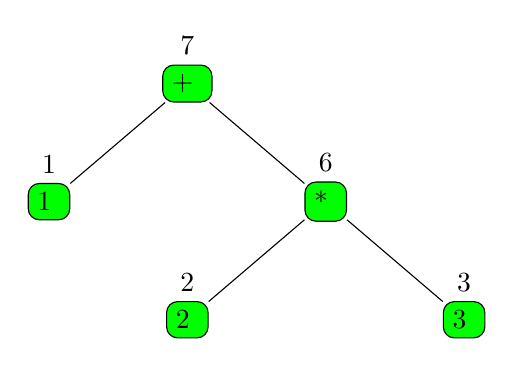
\begin{tikzpicture}[sibling distance=10em, every node/.style = {shape=rectangle, rounded corners, draw, align=center}]]
\node[fill=green, label={7}] { + }
child { node[fill=green, label={1}] { 1 }}
child { node[fill=green, label={6}] { * }
 child { node[fill=green, label={2}] { 2 } }
 child { node[fill=green, label={3}] { 3 } }
}
;
\end{tikzpicture}
\centering
\caption{Syntaxbaum für den Ausdruck \textit{1 + 2 * 3}}
\label{fig:example_syntax_tree}
\end{figure}

\subsection{Token}
\label{sub:token}
Ein Token ist eine Zeichenkette, der innerhalb der lexikalischen Analyse ein Typ (\ac{zb} Zahl, Bezeichner oder Schlüsselwort(\textit{int}, \textit{if}, etc.)) zugewiesen wird.

\subsection{Scanner}
\label{sub:scanner}
Ein Werkzeug, das den Eingabetext in \hyperref[sub:token]{Token} umwandelt. Kann Fehler in der Zeichenabfolge innerhalb eines \hyperref[sub:token]{Token} finden, aber nicht in der Abfolge mehrerer \hyperref[sub:token]{Token}.

\subsection{Parser}
\label{sub:parser}
Ein Werkzeug, das die vom Scanner generierte Abfolge von \hyperref[sub:token]{Token} einliest und validiert. Kann für jede Kombination von \hyperref[sub:token]{Token} eine Aktion auslösen, wie zum Beispiel das Hinzufügen eines Knoten im Syntaxbaum.

%---
\chapter{Problemanalyse}
\label{cha:problemanalyse}

Das Ziel soll es sein, einerseits ein alleinstehendes Programm zur Konvertierung von \hyperref[sub:expression]{Ausdrücken} zu \hyperref[sub:syntax_tree]{Syntaxbäumen} (erstmal nur in Datenform), zu erstellen. Und anderseits ein Web-Interface zum Eingeben der \hyperref[sub:expression]{Ausdrücke} und Betrachten der erzeugten \hyperref[sub:syntax_tree]{Syntaxbäume}. Somit ist die eigentliche Logik des Programms getrennt von der Benutzerschnittstelle. 

Das Programm zur Konvertierung der \hyperref[sub:expression]{Ausdrücke} besteht dann aus den typischen Komponenten eines Compilers: eine Komponente zur Speicherung des \ac{ast}, eine Komponente zur Verwaltung der Symbole (\hyperref[sub:symtab]{Symboltabelle}), generierte \hyperref[sub:scanner]{Scanner} und \hyperref[sub:parser]{Parser} und schließendlich eine Menge von Knotentypen für die einzelnen Operationen.

%---
\chapter{Implementierung}
\label{cha:implementierung}

Die Grundarchitektur (siehe Abbildung \ref{fig:architecture}) des Lösungskonzeptes besteht aus einer klassischen Unterteilung in Front- und Backend. Das Frontend ist für die Datenabfrage und die Darstellung zuständig. Im Backend wiederum steckt die eigentliche Logik des Programms. Da das eigentliche Backend auch als eigenständiges Kommandozeilenprogramm funktionieren soll, wurde die Kommunikation mit dem Frontend auf ein Backend-Interface ausgelagert, die das Kommandozeilenprogramm auf dem Server aufruft und die Resultate zurück an das Frontend schickt. 

\begin{figure}
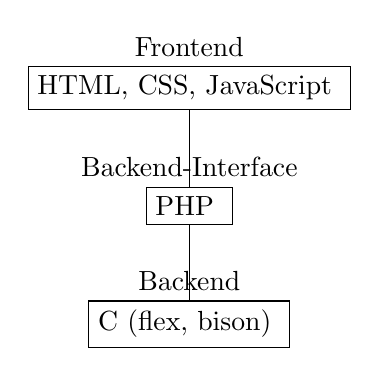
\begin{tikzpicture}[sibling distance=10em, every node/.style = {shape=rectangle, draw, align=center}]]
\node[fill=white, label={Frontend}] { HTML, CSS, JavaScript }
child { node[fill=white, label={Backend-Interface}] { PHP } 
 child { node[fill=white, label={Backend}] { C (flex, bison) } }
}
;
\end{tikzpicture}
\centering
\caption{Grundarchitektur}
\label{fig:architecture}
\end{figure}

\section{Statistiken}
\label{sec:stats}

\subsection{Quellcodestatistiken}
\label{sub:code_stats}
Die Quellcodestatistiken wurden mit dem Tool \textbf{cloc}\footnote{\url{https://github.com/AlDanial/cloc} (Stand 19.02.2020)} erstellt und sind vom aktuellen Projektstand am 19.02.2020.
\begin{table}
\begin{center}
\begin{tabular}{|c || c | c | c | c |} 
 \hline
 \textbf{Language} & \textbf{files} & \textbf{blank} & \textbf{comment} & \textbf{code} \\
 \hline
 JavaScript & 2 & 25 & 3 & 225 \\ 
 \hline
 CSS & 1 & 10 & 0 & 37 \\
 \hline
HTML & 1 & 2 &  0 & 34 \\
 \hline
\hline
SUM & 5 & 37 & 3 & 296 \\
\hline
\end{tabular}
\end{center}
\caption{Quellcodestatistiken zum Web-Interface}
\label{tab:stats_web}
\end{table}

\begin{table}
\begin{center}
\begin{tabular}{|c || c | c | c | c |} 
 \hline
 \textbf{Language} & \textbf{files} & \textbf{blank} & \textbf{comment} & \textbf{code} \\
 \hline
 PHP & 1 & 1 & 0 & 19 \\
 \hline
\hline
SUM & 1 & 1 & 0 & 19 \\
\hline
\end{tabular}
\end{center}
\caption{Quellcodestatistiken zum Backend-Interface}
\label{tab:stats_php}
\end{table}

\begin{table}
\begin{center}
\begin{tabular}{|c || c | c | c | c |} 
 \hline
 \textbf{Language} & \textbf{files} & \textbf{blank} & \textbf{comment} & \textbf{code} \\
 \hline
 C & 18 & 778 & 833 & 4848 \\ 
 \hline
 C/C++ Header & 23 & 139 & 28 & 599 \\
 \hline
yacc & 1 & 45 & 0 & 330 \\
 \hline
lex & 1 & 22 & 0 & 99\\
 \hline
\hline
SUM & 43 & 984 & 861 & 5876 \\
\hline
\end{tabular}
\end{center}
\caption{Quellcodestatistiken zum c-nodes Kommandozeilenprogramm}
\label{tab:stats_backend}
\end{table}

\section{Web-Interface}
\label{sec:frontend}
Das gesamte Frontend besteht aus einer HTML-, einer CSS- und zwei JavaScript-Dateien (eine davon ist die zur Darstellung des \hyperref[sub:syntax_tree]{Syntaxbaum} verwendete \hyperref[sub:d3js]{D3.js Bibliothek}). Die HTML und CSS Dateien sind je unter 50 Quellcodezeilen lang und somit sehr trivial gehalten. In der eigenen JavaScript-Datei werden die Eingaben des Benutzers ausgelesen, formatiert und dann an das Backend geschickt. Die Antwort wird wiederum verwendet um die resultierenden \hyperref[sub:syntax_tree]{Syntaxbäume} zu zeichnen.



\section{Backend-Interface}
\label{sec:backend_interface}
Das Backend-Interface besteht aus einer einzigen PHP-Datei, die im Grunde nichts anderes macht, als das eigentliche Backend mit den Parametern aus der Anfrage des Frontends aufzurufen und die Ergebnisse formatiert wieder ans Frontend zurückzuschicken. Da das Skript sehr kurz ist, habe ich es direkt in diese Dokumentation eingefügt.


\begin{lstlisting}[language=PHP, label={lst:BackendInterface}, caption={Das gesamte Backend-Interface-Skript}]
<?php
	header("Content-Type: application/json");
	$json_output = array();
	$post = file_get_contents('php://input');
	$data = JSON_decode($post, true);
	if( !isset($data['expr'])) {
		# 'leere' Antwort, falls kein Ausdruck übergeben wurde
		echo("{\"expr\":\"\", \"trees\":{}}");
	}
	else {
		# End of line ('\n') Symbole entfernen
		$expr = str_replace(PHP_EOL, '', $data['expr']);
		# Das eigentliche Kommandozeilenprogramm aufrufen und die Ausgabe speichern
		exec("./c-nodes.out -expr \"".$expr."\" -symbols \"".$data['symbols']."\" -json", $json_output);

		echo "{ \"expr\": \"".$expr."\",";
		echo "  \"list\": ";
		# Die Ausgabe Zeile für Zeile zurückgeben
		foreach($json_output as $line) {
			echo $line;
		}
		echo "}";
	}
?>
\end{lstlisting}

\section{c-nodes Kommandozeilenprogramm}
\label{sec:backend}
Der Großteil der Arbeit ist in das Kommandozeilenprogramm \textit{c-nodes} geflossen. Dieses nimmt grundlegend einen Text, bestehend aus Deklarationen und Ausdrücken, und eine optionale Reihe von Symbolen entgegen. Als Resultat gibt das Programm eine Liste der \hyperref[sub:syntax_tree]{Syntaxbäume} in einem der Formate (JSON oder tex) auf der Standardausgabe aus. Alternativ kann die Ausgabe auch direkt in eine angegebene Datei geschrieben werden. Für die Generierung des \hyperref[sub:scanner]{Scanners} wurde hierbei \hyperref[sub:flex]{flex} und für die Generierung des \hyperref[sub:parser]{Parsers} \hyperref[sub:bison]{Bison} verwendet.


\subsection{Codekonventionen}
\label{sub:code_conventions}
\subsubsection{struct / union}
\label{subsub:struct_unions}
Um in C nicht bei jedem Benutzen einer \textit{struct} (im folgenden analog auch \textit{union}), das Schlüsselwort \textit{struct} vor den definierten Typs zu schreiben, ist es verbreitet, ein anonymes \textit{struct} mit \textit{typedef} auf den gewünschten Typnamen zu definieren.
\begin{lstlisting}[label={lst:typedef_struct}, caption={Benennen eines anonymen Typs mit typedef}]
typedef struct {
    int a, b, c;
} MyType;
MyType my_type; // statt 'struct MyType my_type;'
\end{lstlisting}
Die hat allerdings zur Folge, dass das \textit{struct} nun nicht mehr voraus deklariert werden kann.
\begin{lstlisting}[label={lst:typedef_struct_forward_declaration}, caption={Problem beim Vorausdeklarieren eines anonymen Typs}]
// Vorausdeklaration von MyType und eine Funktion, die MyType benutzt
struct MyType;
void func(struct MyType my_type);

// Definition des struct mit typedef
typedef struct {
    int a, b, c;
} MyType;

void func(MyType my_type) { // <= Warnung 'parameter different from declaration'
    ...
}
\end{lstlisting}
Um das zu umgehen, brauchen wir sowohl die \textit{struct}-Definition, als auch den \textit{typedef}, mit dem Namen des \textit{struct}.
\begin{lstlisting}[label={lst:typedef_struct_new}, caption={Lösung zur Definition von structs}]
typedef struct MyType { 
    int a, b, c;
} MyType;
\end{lstlisting}
Zwar wird in diesem Projekt keine Vorausdeklaration von \textit{struct}s benutzt, jedoch wird diese Konvention benutzt um bei einer eventuellen Erweiterung dies zu ermöglichen. \textbf{Dieses Vorgehen gilt auch analog für die Definition von \textit{union}s.}

\subsection{Implementierung des Scanners}
\label{sub:impl_scanner}
Als Grundlage für den \hyperref[sub:scanner]{Scanner} wurde die \textbf{Lex-Spezifikation}\footnote{\url{https://www.lysator.liu.se/c/ANSI-C-grammar-l.html} (Stand 19.02.2020)} von Jutta Degener genutzt, aber alle nicht für die Implementierung benötigten Tokens (\ac{zb} \textit{volatile}, \textit{auto} oder \textit{static}) entfernt. Allerdings wurde statt lex das modernere \hyperref[sub:flex]{flex} zur Generierung des \hyperref[sub:scanner]{Scanners} benutzt.

\subsection{Implementierung des Parsers}
\label{sub:impl_parser}
Analog zur \hyperref[sub:impl_scanner]{Implementierung des Scanner} wurde die \textbf{Yacc-Spezifikation}\footnote{\url{https://www.lysator.liu.se/c/ANSI-C-grammar-y.html} (Stand 19.02.2020)} von Jutta Degener als Basis genutzt, und auch an den Umfang dieses Projektes angepasst. Auch hier wurde der Generator yacc durch das modernere \hyperref[sub:bison]{Bison} ersetzt.

\subsection{Repräsentation von Datentypen und Werten}
\label{sub:value_types}
Jeder Knoten hat genau einen Datentyp, der entweder beim Erschaffen des Knoten (\ac{zb} Konstanten) festgelegt oder bei der semantischen Analyse von den Kindknoten abgeleitet wird. Bei letzter Art von Knoten wird der Datentyp beim Erschaffen auf den Datentyp \textit{VT\_ERROR} gesetzt. Gibt es nach der semantischen Analyse noch Knoten mit dem Datentyp \textit{VT\_ERROR} wird die Interpretation des \hyperref[sub:syntax_tree]{Syntaxbaums} nicht gestartet. Die verfügbaren Datentypen sind wie folgt definiert:
\begin{lstlisting}[label={lst:ValueType}, caption={ValueType}]
typedef enum ValueType {
    VT_ERROR = 0,
    VT_INT = 1,
    VT_DOUBLE = 2,
} ValueType;
\end{lstlisting}
Die einzelnen Werte repräsentieren hierbei Bits, \ac{dh} würde ein weiterer Datentyp hinzukommen (\ac{zb} \textit{char}) bekäme dieser den Wert $2^2 = 4$.Kein gesetztes Bit repräsentiert keinen "`richtigen"' Datentyp bzw. den Datentyp \textit{VT\_ERROR}. Dies wurde so gewählt damit Datentypen mit Bitoperationen einfach kombiniert werden können. Darauf wird im Abschnitt \hyperref[sub:node]{Knoten} genauer eingegangen.

Um nicht für jeden Datentyp eine Variable für den jeweiligen Wert zu definieren (jeweils eine Variable für die Datentypen \textit{int} und \textit{double}), wurden die Werte in einer \textit{union} zusammengefasst:
\begin{lstlisting}[label={lst:Value}, caption={Value}]
typedef union Value {
    int i_value;
    double d_value;
} Value;
\end{lstlisting}
Somit ist immer nur ein Wert "`aktiv"'. Der Speicherbedarf für alle Werte ist hierbei immer der Speicherbedarf des größten Datentyps (hier \textit{double} mit 8 Bytes). Nachteil bei diesem Vorgehen ist, dass \ac{zb} \textit{i\_value} gesetzt, aber \textit{d\_value} ausgelesen wird. Um das zu verhindern muss immer ein \hyperref[lst:ValueType]{ValueType} mit einem \hyperref[lst:Value]{Value} assoziiert werden, der den zu benutzenden Wert bestimmt.

\subsection{Knoten}
\label{sub:node}
Jeder Knoten hat genau einen \textbf{Ausgang} und bis zu drei \textbf{Eingänge}, aus denen der Ausgangswert und -typ berechnet wird. Häufig wird auch \textbf{Kindknoten} und \textbf{Elternknoten} als Begriffe bei Bäumen verwendet. Bei dem hier verwendeten Modell entsprechen die \textbf{Kindknoten} den \textbf{Eingängen}, und die Knoten kennen ihren Elternknoten nicht. Hier wurde mit Absicht von der üblichen Benennung Abstand genommen, um deutlich zu machen, dass ein Knoten keinerlei Einfluss auf die Funktionsweise oder die Werte seiner \textbf{Eingänge} hat und nur Daten bereitstellt, die von einem eventuellen \textbf{Elternknoten} benutzt werden können. Der Knoten an sich hat aber keine Verbindung zu seinem \textbf{Elternknoten} und funktioniert unabhängig von dessen Funktion. Die genaue Funktionsweise wird in den Sektionen \hyperref[sub:node_out]{Knotenausgang} und \hyperref[sub:node_in]{Knoteneingänge} erläutert.

\begin{lstlisting}[label={lst:Node}, caption={Node}]
typedef struct Node {
    NodeIn in; 
    NodeOut out;
    bool (*processNode)(Node* node, const ProcessMode process_mode);
    char text[20];
    char error[200];
    void* additional_info;
    SymbolHandle symbol_handle;
} Node;
\end{lstlisting}

\textit{processNode} ist ein Funktionszeiger auf eine Funktion, die den jeweiligen Knoten verarbeiten kann (siehe als Beispiel \hyperref[lst:processNode]{processNode\_GetSymbol}). In \textit{text} wird der Namen des Knoten gespeichert, welcher in den allermeisten Fällen dem vom Scanner erzeugten Token entspricht (\ac{zb} \textbf{+} für einen Additionsknoten). In \textit{error} wird eine eventuelle Fehlernachricht zu einem Fehler, der bei diesem Knoten aufgetreten ist, gespeichert. \textit{additional\_info} ist ein Zeiger auf einen nicht näher spezifierten Datenblock und kann für verschiedene Dinge benutzt werden (\ac{zb} um eine Referenz zur \hyperref[sub:impl_symtab]{Symboltabelle} zu speichern). In \textit{symbol\_handle} kann ein Verweis zu einem Symbol gespeichert werden (standardmäßig auf \textit{0 / kein Symbol} gesetzt).

\subsubsection{Knotenausgang}
\label{sub:node_out}
Im Ausgang eines Knotens werden primär der Datentyp und der Wert des Knoten gespeichert. Dazu gibt es noch die Metadaten \textit{is\_lvalue} (gibt an, dass der Knoten auf ein manipulierbares Symbol verweist) und \textit{is\_processed} (gibt an, ob der Knoten schon verarbeitet wurde, um \ac{zb} Mehrfachverarbeitung zu verhindern). All diese Daten werden einerseits vom Elternknoten als Eingangsdaten, und anderseits zur Darstellung des Knoten im \hyperref[sub:syntax_tree]{Syntaxbaum}, benutzt.
\begin{lstlisting}[label={lst:NodeOut}, caption={NodeOut}]
typedef struct NodeOut {
    ValueType   type;
    Value       value;
    bool        is_lvalue;
    bool        is_processed;
} NodeOut;
\end{lstlisting}

\subsubsection{Knoteneingänge}
\label{sub:node_in}
In einem Eingangsslot wird ein Verweis auf einen Knoten und dazugehörige Metadaten gespeichert. In \textit{allowed\_value\_types} wird eine Bitmaske für die \hyperref[sub:value_types]{ValueTypes} gespeichert, mit der abgeglichen wird, ob ein Eingangsknoten den richtigen Ausganstyp hat. Dazu werden die jeweiligen \hyperref[sub:value_types]{ValueTypes} einfach mit einem binären Oder-Operator verknüpft.
\begin{lstlisting}[label={lst:InSlot}, caption={InSlot}]
typedef struct InSlot {
    Node* node;
    uint32_t allowed_value_types;
    bool allow_rvalues;
} InSlot;
\end{lstlisting}

\begin{lstlisting}[label={lst:allowed_value_types}, caption={Verknüpfen von ValueTypes}]
slot_0.allowed_value_types = VT_INT; // nur 'int' erlaubt
slot_1.allowed_value_types = VT_INT | VT_DOUBLE; // 'int' und 'double' erlaubt
\end{lstlisting}
\textit{allow\_rvalues} gibt an, ob der Eingang \hyperref[sub:lvalues_rvalues]{rvalues} als Eingang akzeptiert oder nicht. Meistens ist dies auf \textit{true} gesetzt, Ausnahmen wären der Zuweisungsoperator(\textbf{=}) oder die Inkrement-/Dekrementoperatoren(\textbf{++}, \textbf{--}), die zwingend einen \hyperref[sub:lvalues_rvalues]{lvalue} brauchen, den sie manipulieren können.

Jeder Knoten kann bis zu 3 \hyperref[lst:InSlot]{Eingangsslots} haben, die konkrete Anzahl der Eingänge wird in \textit{slot\_count} gespeichert. Auf die jeweiligen  \hyperref[lst:InSlot]{Slots} kann man entweder einzeln (\textit{slot\_0}, \textit{slot\_1} und \textit{slot\_2}) oder iterativ (\textit{slot[i]}) zugreifen.
\begin{lstlisting}[label={lst:NodeIn}, caption={NodeIn}]
typedef struct NodeIn {
    union {
        struct {
            InSlot slot_0;
            InSlot slot_1;
            InSlot slot_2;
        };
        InSlot slot[3];
    };
    uint8_t slot_count;
} NodeIn;
\end{lstlisting}

\subsubsection{Definition eines Knotentyps}
\label{subsub:node_type_definition}
Für jeden Knotentyp (\ac{dh} für jede Operation und noch ein paar zusätzliche) werden zwei Funktionen benötigt. Einerseits eine Funktion, die den Knoten verarbeitet (\textit{processNode\_<Knotentyp>}) und anderseits eine Funktion die den Knoten erschafft (\textit{createNode\_<Knotentyp>}, also alle benötigten Parameter eines \hyperref[lst:Node]{Nodes} festlegt.

Als Beispiel wird hier die Verarbeitungsfunktion des Knotens zum Abrufen eines Symbols gezeigt, da diese relativ kompakt in der Länge, aber doch relativ umfangreich bei den benutzten Parametern ist. \textit{process\_mode} gibt hierbei an, ob die Verarbeitung nur den Datentyp des Knoten bestimmen (\textbf{PM\_TYPE\_ONLY}), also im Prinzip die semantische Analyse, oder den Knoten komplett verarbeiten soll (\textbf{PM\_FULL}), also auch die restlichen Werte verändern.
\begin{lstlisting}[label={lst:processNode}, caption={processNode\_GetSymbol}]
bool processNode_GetSymbol(Node* node, const ProcessMode process_mode) {
    SymbolTable* sym_tab = (SymbolTable*) node->additional_info;
    if(!sym_tab) {
        strcpy(node->error, "DEBUG: No reference to symbol table");
        return false;
    }
    SymbolHandle handle = getSymbolHandle(sym_tab, node->text);
    if(handle.value == 0) {
        sprintf(node->error, "There's no variable named '%s'", node->text);
        return false;
    }
    SymbolValue sym_value = getSymbolValue(sym_tab, handle);
    node->out.type = sym_value.type;
    if(process_mode == PM_FULL) {
        node->out.is_lvalue = !sym_value.is_const; 
        node->symbol_handle = handle;
        node->out.value = sym_value.value;
    }
    return true;
}
\end{lstlisting}
Und folgend die Erstellungsfunktion des Knoten, die die Verarbeitungsfunktion mit dem Knoten verknüpft und die restlichen Parameter des \hyperref[lst:Node]{Nodes} initial setzt.
\begin{lstlisting}[label={lst:createNode}, caption={createNode\_GetSymbol}]
Node createNode_GetSymbol(const char* identifier) {
    Node node = {
        .in = {
            .slot_count = 0,
        }, 
        .out = {
            .type = VT_ERROR,
            .value.i_value = 0,
            .is_lvalue = false,
            .is_processed = false,
        },
        .processNode = processNode_GetSymbol,
        .additional_info = NULL,
        .error = "",
        .symbol_handle = 0,
    };
    strcpy(node.text, identifier);
    return node;
}
\end{lstlisting}

\subsection{Abstrakter Syntaxbaum (AST)}
\label{sub:impl_ast}
In der Implementierung wird der \ac{ast} nur als Speicherverwaltung für die \hyperref[sub:node]{Knoten} benutzt.
\begin{lstlisting}[label={lst:AbstractSyntaxTree}, caption={AbstractSyntaxTree}]
#define AST_MAX_NODES 256

typedef struct AbstractSyntaxTree {
    Node nodes[AST_MAX_NODES];
    uint16_t node_count;
} AbstractSyntaxTree;
\end{lstlisting}
Dazu gibt es noch eine Reihe von "`makeNode"'-Funktionen, um die \hyperref[sub:node]{Knoten} in den \ac{ast} einzufügen. Diese folgen alle dem gleichen Schema und haben als Parameter mindestens einen Zeiger auf ein \hyperref[lst:AbstractSyntaxTree]{AbstractSyntaxTree}-Objekt und eine Knotenerstellungsfunktion. Zusätzlich kann es noch mehr Parameter geben, die zur Erstellung eines Knoten benötigt werden.
\begin{lstlisting}[label={lst:makeNode}, caption={Auswahl verschiedener "`makeNode"'-Funktionen}]
Node* makeNode_0(AbstractSyntaxTree* ast, Node (*createNode)(void));
Node* makeNode_1(AbstractSyntaxTree* ast, Node (*createNode)(Node* node_0), Node* node_0);
Node* makeNode_0_INT(AbstractSyntaxTree* ast, Node (*createNode)(const int value), const int value);
Node* makeNode_2_STRING(AbstractSyntaxTree* ast, Node (*createNode)(Node* node_0, Node* node_1, const char* value), Node* node_0, Node* node_1, const char* value);
Node* makeNode_0_SymbolValue(AbstractSyntaxTree* ast, Node (*createNode)(SymbolValue value), SymbolValue value);
\end{lstlisting}

Die jeweiligen "`makeNode"'-Funktionen erzeugen dann mit der übergebenen Knotenerstellungsfunktion (siehe Listing \ref{lst:makeNode_use}), und den eventuellen zusätzlichen Parametern, ein \hyperref[lst:Node]{Node}-Objekt und fügen es der Liste des \hyperref[lst:AbstractSyntaxTree]{AbstractSyntaxTree}-Objekt hinzu:
\begin{lstlisting}[label={lst:makeNode}, caption={Auswahl der "`makeNode"'-Funktionen}]
Node* makeNode_2_STRING(AbstractSyntaxTree* ast, Node (*createNode)(Node* node_0, Node* node_1, const char* value), Node* node_0, Node* node_1, const char* value) {
    if(ast->node_count < AST_MAX_NODES) {
        ast->nodes[ast->node_count++] = createNode(node_0, node_1, value);
        PRINT_DEBUG("Inserted node from makeNode_2_STRING on #%d\n", ast->node_count-1);
        return &(ast->nodes[ast->node_count-1]);
    }
    PRINT_DEBUG("Failed to insert node from makeNode_2_STRING");
    return NULL;
}
\end{lstlisting}

\begin{lstlisting}[label={lst:makeNode_use}, caption={Verknüpfung von "`makeNode"'- und "`createNode"'-Funktionen mit Parametern}]
Node* node = makeNode_0_STRING(&ast, createNode_GetSymbol, $1); 
\end{lstlisting}

\subsection{Symboltabelle}
\label{sub:impl_symtab}
\subsubsection{Symbolattribute}
\label{subsub:impl_symbols}
Je nach Ansicht ist der Typqualifizierer (\textit{const} oder \textit{volatile}(nicht implementiert)) Teil des Datentyp oder ein extra Attribut. In der Implementierung wird der vereinfachte Typqualifizierer (\textit{const} oder \textit{nicht const}) als extra Symbolattribut behandelt.
Beispiele:

\begin{table}
\begin{center}
\begin{tabular}{|c || c | c | c | c |} 
 \hline
 \textbf{Symboldefinition} & \textbf{Name} & \textbf{Datentyp} & \textbf{Wert} & \textbf{Typqualifizierer} \\
 \hline
 const int a = 2 & a & int & 2 & const \\ 
 \hline
 double b & b & double & ? / 0.0 & - \\
 \hline
\end{tabular}
\end{center}
\caption{Beispiele von Symbolen}
\label{tab:symbols}
\end{table}
Da es keine Namensräume in der Implementierung gibt, werden alle Symbole als global angesehen, \ac{dh} ein nicht initialisiertes Symbol mit Datentyp \textit{int} bekommt den Wert \textit{0}, analog dazu \textit{0.0} für ein \textit{double}.

Die Symbolattribute (ohne den \hyperref[sub:identifier]{Bezeichner}) werden im \textit{struct} \hyperref[lst:SymbolValue]{SymbolValue} zusammengefasst. Dazu gehören der Datentyp, der Wert und der (vereinfachte) Typqualifizierer.
\begin{lstlisting}[label={lst:SymbolValue}, caption={SymbolValue}]
typedef struct SymbolValue {
    ValueType type;
    Value value;
    bool is_const;
} SymbolValue;
\end{lstlisting}

\subsubsection{Die Tabelle}
\label{subsub:impl_table}
Ein \hyperref[lst:SymbolHandle]{SymbolHandle} ist im Prinzip nur ein einfacher Index in der Symboltabelle, der auf ein bestimmtes Symbol verweist, wobei der Wert \textbf{0}, ähnlich wie bei Zeigern, für kein Symbol bzw. ein ungültiges Symbol steht.
\begin{lstlisting}[label={lst:SymbolHandle}, caption={SymbolHandle}]
typedef struct SymbolHandle {
    uint8_t value;
} SymbolHandle;
\end{lstlisting}
 Man hätte hier auch einen einfachen \textit{typedef} benutzen können: \lstinline[columns=fixed]{typedef uint8_t SymbolHandle;}. Allerdings könnte es hier in Zukunft Probleme bei weiteren ähnlich definierten \textit{Handles} geben:
\begin{lstlisting}[label={lst:about_handles}, caption={Problem beim Definieren von "`Handle"'-typen mit typedef}]
typedef uint8_t SymbolHandle;
typedef uint8_t AnotherHandle;

void useSymbolHandle(SymbolHandle handle) {...}

AnotherHandle another_handle = 5;
useSymbolHandle(another_handle); // Der Compiler sieht hier keinen Typunterschied mehr
\end{lstlisting}
Mit der benutzten Methode ist ein unabsichtliches Verwechseln von verschiedenen \textit{Handletypen} quasi nicht mehr möglich.

\begin{lstlisting}[label={lst:SymbolTable}, caption={SymbolTable}]
#define MAX_SYMBOL_LENGTH 20
#define MAX_SYMBOLS 64
typedef struct SymbolTable {
    char identifiers[MAX_SYMBOL_LENGTH][MAX_SYMBOLS];
    SymbolValue values[MAX_SYMBOLS];
    uint8_t symbol_count;
    SymbolValue currentConfig;
} SymbolTable;
\end{lstlisting}
Die \hyperref[lst:SymbolTable]{SymbolTable} speichert primär zwei gleich große Arrays, mit einerseits den Bezeichnern und anderseits den Symbolattributen. Bezeichner und Symbolattribute werden einfach über den gleichen Index verbunden. So gehört der \hyperref[lst:SymbolValue]{SymbolValue} bei \textit{values[2]} zu dem Bezeichner bei \textit{identifiers[2]}. \textit{symbol\_count} gibt die Gesamtzahl der gespeicherten Symbole an. \textit{currentConfig} wird benutzt um neue Bezeichner mit einer bestimmten Konfiguration der Symbolattribute hinzuzufügen.

%---
\chapter{Evaluierung}
\label{cha:evaluation}
Auf Seiten der Funktionalität des Werkzeugs wurden die Ziele der Arbeit vollständig erreicht oder sogar teilweise übertroffen. Benutzer können nun statt, wie geplant, nur einen einzelnen Ausdruck, regulären ANSI-C Quellcode (mit Einschränkungen bezüglich Programmsteuerungsanweisungen, Zeigern, Arrays, etc.) in das Werkzeug eintragen und sich die Syntaxbäume aller Ausdrücke anzeigen lassen.

Jedoch war leider keine Zeit mehr, das enstandene Werkzeug von den Programmieranfängern testen und evaluieren zu lassen. Dies wird allerdings im nächsten Semester nachgeholt und die Ergebnisse dieser Evaluation dokumentiert, so dass sie eventuell eine Basis für eine weitere Projektarbeit stellen, die sich mit der Erweiterung dieses Werkzeugs befasst.

%---
\chapter{Zusammenfassung und Ausblick}
\label{cha:zusammenfassung}
\section{Erreichte Ergebnisse}
\label{sec:ergebnisse}

Wie in Abbildung \ref{fig:result} zu sehen ist, wurde mit dem Werkzeug das Ziel der Arbeit erreicht und man kann sich auch für komplexere \hyperref[sub:expression]{Ausdrücke}, einen \hyperref[sub:syntax_tree]{Syntaxbaum} mit farbig kodierten Typinformationen und Werten für jeden einzelnen Knoten, darstellen lassen.

\begin{figure}[htbp]
  \centering
  \includegraphics[width=0.8\textheight]{images/result.jpg}
  \caption{Syntaxbaum eines komplexeren Ausdrucks}
  \label{fig:result}
\end{figure}

\section{Ausblick}
\label{sec:ausblick}

\subsection{Erweiterbarkeit der Ergebnisse}
\label{sub:erweiterbarkeit}

\subsubsection{Hinzufügen weiterer primitiver Datentypen (char, long, bool, float, etc.)}
Prinzipiell dürfte das Hinzufügen weiterer primitiver Datentypen keine großen Probleme bereiten, jedoch müsste so gut wie jeder \textit{Node} angepasst werden, um mit dem neuen Datentyp umgehen zu können.
\begin{itemize}
\item{Schwierigkeit: Gering}
\item{Aufwand: Mittel}
\end{itemize}
\subsubsection{Felder als Datentyp}
\label{subsub:arrays}
Für die Implementierung von Feldern müsste auf jeden Fall die Symboltabelle überarbeitet werden. Ein einfacher Weg wäre hier zum Beispiel die Definition von 10 \textit{int}-Symbolen mit automatisch generierten Namen für ein \textit{int}-Feld der Größe 10. Wenn wir dann nur von einfachen Lese- und Schreiboperationen mithilfe des Index-Operators \textit{[]} auf die einzelnen Datenfelder ausgehen, würde sich der Aufwand bei den \textit{Nodes} hier wohl auf eine Anpassung des Lese-\textit{Nodes} von Variablen und dem Zuweisungs-\textit{Nodes} beschränken. Da die Speicherreservierung bisher jedoch nicht zwingend linear erfolgt, müsste wahrscheinlich extra Aufwand betrieben werden um zu garantieren, dass alle Elemente des Feldes in einem Block liegen und auch der Zugriff auf das (n+1)-te Element eines Feldes, den "`richtigen"' Effekt hat, also den Speicherbereich nach dem eigentlichen Feld ausliest bzw. manipuliert.
\begin{itemize}
\item{Schwierigkeit: Mittel}
\item{Aufwand: Mittel}
\end{itemize}
\subsubsection{Zeiger als Datentyp}
Wahrscheinlich dürfte es reichen ein weiteres Attribut zu der Definition der Symboltabellenwerte hinzuzufügen. Zum Beispiel \textit{is\_pointer}, wobei der \textit{ValueType} dann auf den referenzierten Datentyp verweist, als Wert jedoch die Adresse im \textit{i\_value} abgespeichert wird. Somit wären Adressen jedoch auf den Wertebereich eines \textit{int} limitiert. Zusätzlich müssten natürlich noch die unären Operatoren \textit{\&} und \textit{*} im  \hyperref[sub:parser]{Parser} implementiert werden.
\begin{itemize}
\item{Schwierigkeit: Mittel}
\item{Aufwand: Mittel}
\end{itemize}
\subsubsection{Zeigerarithmetik}
Zeigerarithmetik (Berechnung der Zeigeradresse inklusive Inkrement und Dekrement) benötigt eine Emulation des Speichers und somit grundlegende Änderungen an mehreren Basissystemen (zum Beispiel an der Symbol Tabelle). Der Aufwand hierfür überschneidet sich mit dem Aufwand zur (vollständigen) Implementierung von \hyperref[subsub:arrays]{Feldern}.
\begin{itemize}
\item{Schwierigkeit: Hoch}
\item{Aufwand: Hoch}
\end{itemize}
\subsubsection{Hinzufügen von Programmsteuerungsanweisungen (Verzweigungen, Schleifen)}
Das Hinzufügen von Programmsteuerungsanweisungen übertrifft bei Weitem die Ursprungsfunktionalität eines Ausdruckauswerters und geht dann schon Richtung eines vollständigen Interpreters. Wahrscheinlich müssten dafür große Teile des bestehenden Projektes angepasst werden.
\begin{itemize}
\item{Schwierigkeit: Hoch}
\item{Aufwand: Sehr hoch}
\end{itemize}
\subsubsection{Bearbeiten des Syntaxbaums...}
Das Bearbeiten des Syntaxbaums im Frontend müsste mit der \hyperref[sub:d3js]{D3.js}-Bibliothek möglich sein, jedoch habe ich mich im Rahmen dieser Arbeit nicht weiter damit befasst.
\begin{itemize}
\item{Schwierigkeit: Nicht einschätzbar}
\item{Aufwand: Nicht einschätzbar}
\end{itemize}
\subsubsection{...und Generieren des entstandenen \textit{C}-Ausdrucks}
Das Generieren des \textit{C}-Ausdrucks aus einem Syntaxbaum besteht größtenteils nur aus Textkonkatenation der Namen der einzelnen Knoten. Bei einzelnen Knoten (zum Beispiel der ternäre Operator oder Funktionen mit Parametern) ist etwas mehr Aufwand von Nöten.
\begin{itemize}
\item{Schwierigkeit: Gering}
\item{Aufwand: Gering}
\end{itemize}

%\subsection{Übertragbarkeit der Ergebnisse}
%\label{sub:uebertragbarkeit}

%-----------------------------------------------------------------------
\appendix

%---
\printbibliography

%---
%\chapter{Anhang A}

%---
%\chapter{Anhang B}


\end{document}